\documentclass{rapportENS}
\title{Title page}
\begin{document}

%----------- Informations du rapport ---------
\titre{Ensemble Domotique EnOcean}
\Departement{Département Mécatronique}
\annee{$1^{ère}$ année}
\sujet{Analyse de système mécatronique }
\enseignant{S. Gardette, O. Bordron,\\ Q. Delamare, Alyssia Dong,\\
R. Le Goff latimier}
\eleves{Adrien \textsc{Vigné} \\ Martin \textsc{Filliung}}

%----------- Initialisation -------------------
\fairemarges{Vigné-Filliung} %Afficher les marges
\fairepagedegarde %Créer la page de garde
\tabledematieres %Créer la table de matières

%------------ Corps du rapport ----------------

\part{Système étudié}
 \section{Présentation du système}
 La domotique a pour but d'interconnecter des sous-systèmes à la base indépendants afin d'améliorer l'interaction de l'ensemble avec l'utilisateur. Ces technologies se retrouvent principalement dans l'habitat grâce à des capteurs connectés, des passerelles de contrôle ainsi que des actionneurs ou des boîtiers de commande afin d'automatiser certaines actions ou de créer des alertes ou routines pour assister l'utilisateur. Ces installations demandent d'être penser à la conception de la maison ou d'entreprendre des modifications afin de pouvoir les adapter à une installation existante car ils nécessitent entre autre une source d'énergie et ont un encombrement non négligeable. L'objet de cette étude a vocation à palier à ces défauts en proposant une solution sans fils, sans alimentation externe et relativement peu encombrante afin de s'ajouter simplement à toute installation existante sans grandes contraintes. 
 
 \section{Caractéristiques du système}
 \subsection{Objectifs du système}

 Cette ensemble domotique est l'ensemble proposé par la société \textit{EnOcean} (figure \ref{fig:kit_enOcean}) avec des modules utilisant le principe de récupération d'énergie afin de minimiser leur impact sur l'installation déjà présente. Le principe de récupération d'énergie est de permettre une indépendance énergétique des modules au travers de transducteurs, tout en remplissant leurs objectifs d'interconnexion. Deux technologies employées pour répondre à ce critère seront étudiées dans ce rapport. 
 
 \begin{figure}[h!]
     \centering
     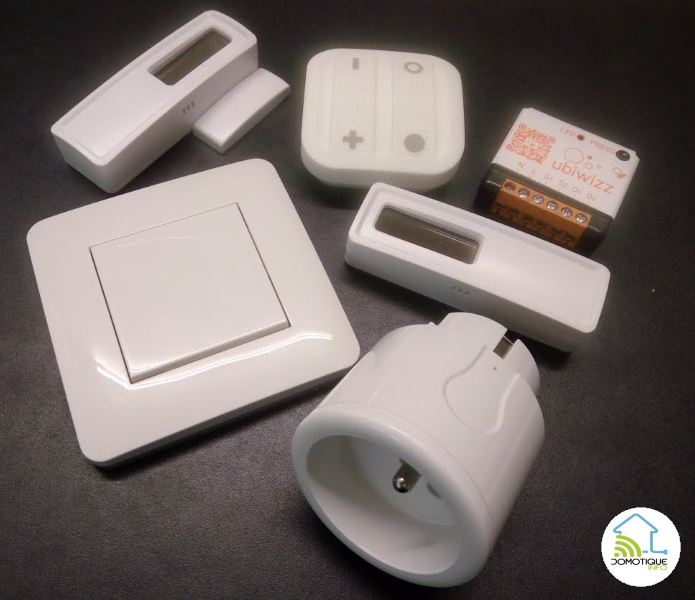
\includegraphics[scale=0.5]{kit_enocean.jpg}
     \vspace{0.5cm}
     \caption{Ensemble de modules \textit{EnOcean}}
     \label{fig:kit_enOcean}
 \end{figure}
 
 \subsection{Cahier des charges}
 Les fonctions principales du kit sont représentées dans un diagramme des interacteurs (Figure \ref{fig:Inter-acteurs}-\ref{tableau_cdcf}) dans le but ici de visualiser les principales fonctionnalités de l'objet d'étude et les contraintes s'appliquant sur celui-ci.
 
 \vspace{0.7cm}
 
 \begin{figure}[h!]
     \centering
     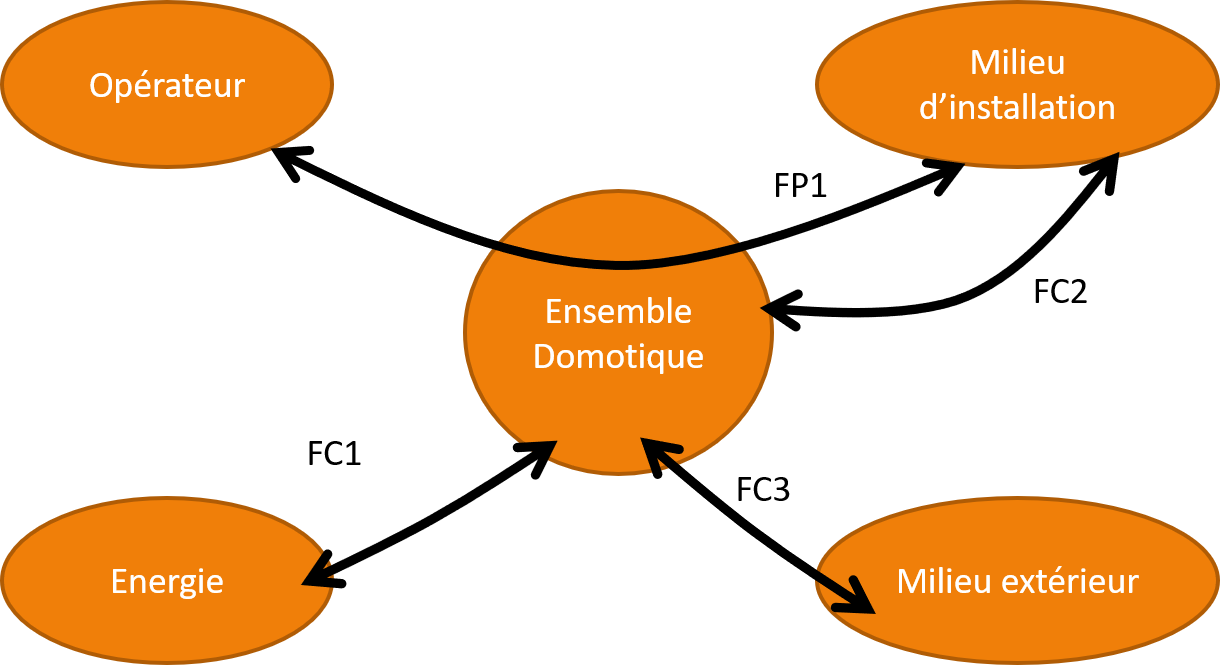
\includegraphics[width=0.9\linewidth]{Graphe_cdcdf.png}
     \vspace{0.7cm}
     \caption{Diagramme des interacteurs}
     \label{fig:Inter-acteurs}
 \end{figure}
 
  \vspace{0.5cm}
 
 \begin{figure}[h!]
    \centering
    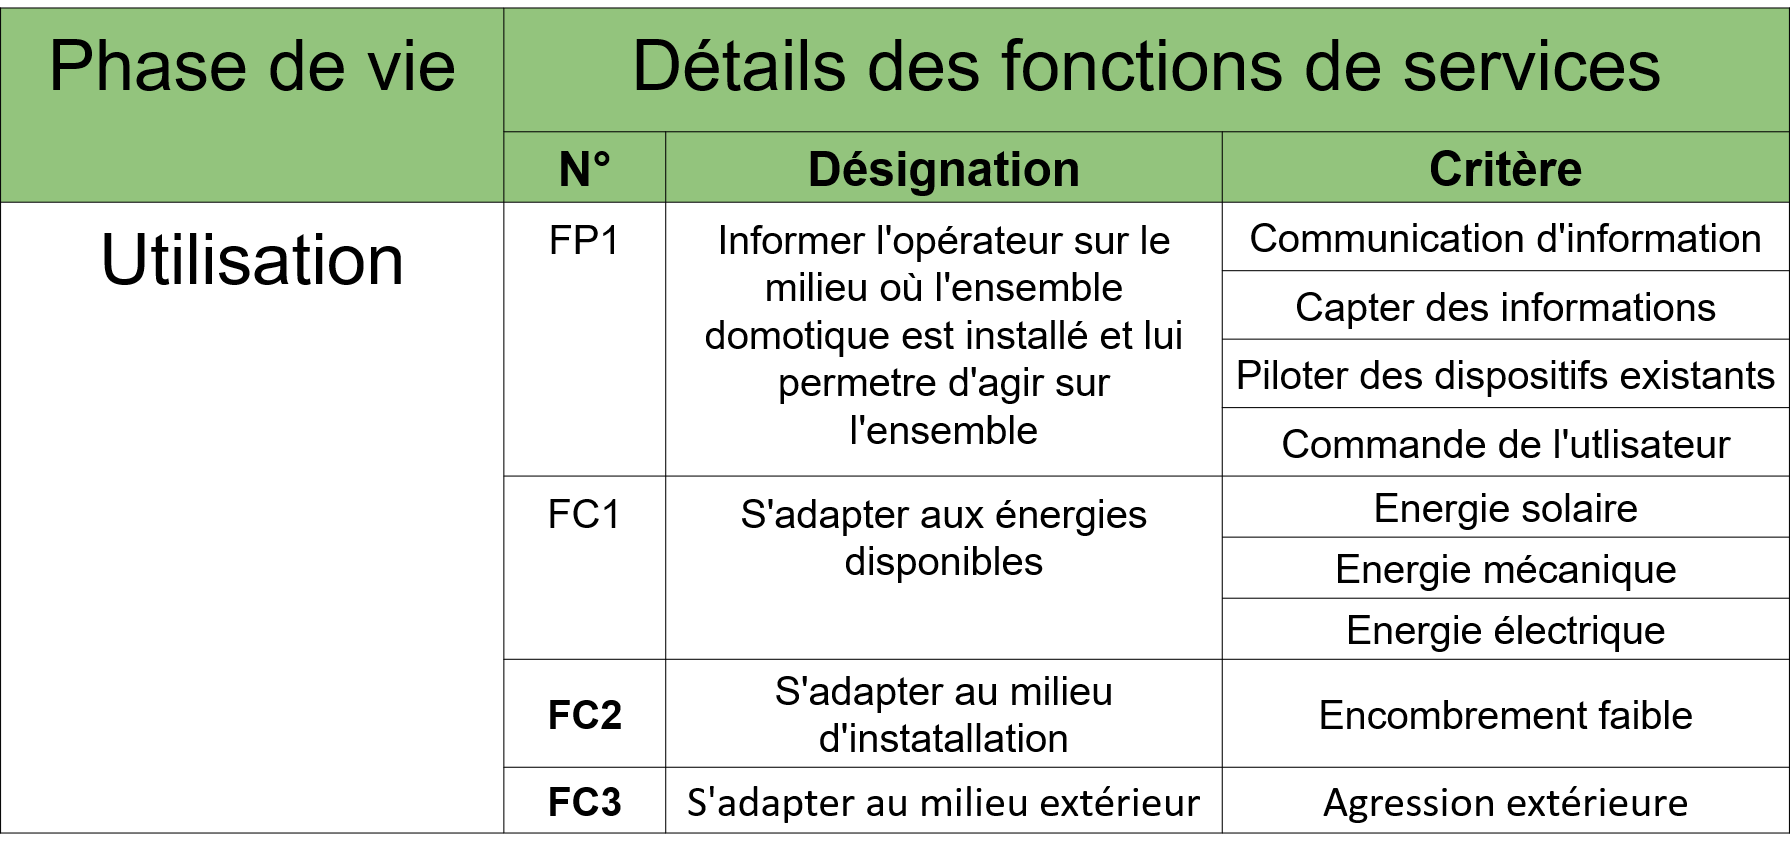
\includegraphics[width=\linewidth]{tableau_cdcf.png}
    \vspace{0.2cm}
    \caption{Tableau du cahier des charges}
    \label{tableau_cdcf}
 \end{figure}

\subsubsection{Contraintes de conception}
La principale contrainte de conception de ce système est la récupération d'énergie ceci imposant la conception ou l'utilisation d'un transducteur afin de récupérer l'énergie nécessaire au fonctionnement du dispositif. Une autre contrainte importante est l'adaptation du dispositif au milieu d'installation notamment au niveau de son encombrement et de sa facilitée de mise en place. La résistance du matériel en milieu extérieur implique aussi un minimum d'étanchéité de celui-ci afin de supporter la pluie et l'humidité notamment.

\subsection{Ensemble disponible pour l'étude}
Afin de mener cette analyse, le kit est composé de :
\vspace{0.1cm}
\begin{itemize}
\item[•] commandes : 
\vspace{0.1cm}
\begin{itemize}
    \item interrupteurs sans fils gradateur;
    \item interrupteurs sans fils monostable.
\end{itemize}
\vspace{0.1cm}
\item[•] capteurs:
\vspace{0.1cm}
\begin{itemize}
    \item 2 capteurs de température;
    \item 1 capteur d'ouverture de porte.
\end{itemize}
\vspace{0.1cm}
\item[•] actionneurs :
\vspace{0.1cm}
\begin{itemize}
    \item 1 prise piloté;
    \item 1 contacteur piloté.
\end{itemize}
\vspace{0.1cm}
\item[•] passerelles : 
\vspace{0.1cm}
\begin{itemize}
    \item 1 passerelle wifi pour tableau électrique;
    \item 1 passerelle pour \textit{Raspberry Pi};
    \item 2 passerelles USB.
\end{itemize}
\vspace{0.1cm}
\item[•] 1 kit de développement  
%  \item plusieurs interrupteurs sans piles 2 canaux;
%  \item 2 capteurs de température et d'hydrométrie;
%  \item 1 capteur d'ouverture de porte / fenêtre;
%  \item 1 contacteur piloté;
%  \item 1 passerelle \textit{EnOcean};
%  \item 1 kit de développement;
%  \item 1 passerelle pour \textit{Raspberry Pi}. 
\end{itemize} 
\vspace{0.1cm}

L'analyse a pour but de vérifier les fonctions principales et de contraintes identifiées ainsi que les caractéristiques techniques annoncées par le constructeur. 
 
%  \section{Caractéristiques du système}
 
%  Les modules proposés par \textit{ubiwizz} sur très variés (Environ 180 articles listés). Mis a notre disposition sont :
%  \begin{itemize}
%  \item plusieurs interrupteurs sans piles 2 canaux;
%  \item plusieurs capteurs de température et d'hydrométrie;
%  \item un capteur d'ouverture de porte / fenêtre;
%  \item un contacteur piloté;
%  \item une passerelle \textit{EnOcean};
%  \item un kit de développement;
%  \item une passerelle programmable \textit{Raspberry Pi}. 
% \end{itemize}  
 
%  \section{Contraintes de conception}
 
%  Les différents modules on pour contrainte d'être entièrement autonome une fois installés : ils ne doivent pas avoir à être rechargés, réinitialisés manuellement ou autrement manipulés pour bien fonctionner. De plus les modules doivent s'intégrer le plus facilement possible à l'environnement dans lequel on les place et donc être miniaturisés.

\subsection{Cas d'utilisation}

Cet ensemble présente plusieurs cas d'utilisation en fonction de l'utilisateur et du produit possédé : 
\vspace{0.1cm}

\begin{itemize}
    \item Le kit de développement (Figure \ref{dev}) permet à un professionnel d'utiliser la plate-forme de communication \textit{EnOcean} avec ses propres capteurs, actionneurs, etc...;
    \item Un kit de design (Figure \ref{aestetics}) qui permet à un professionnel d'utiliser les produits \textit{EnOcean} tout en personnalisant son aspect esthétique;
    \item Les produits des catégories <<commandes>> et <<actionneurs>> peuvent être appairés et servir d'interrupteur portatif à un appareil n'en possédant pas;
    \item La passerelle permet de créer un réseau entre les différents capteurs actionneurs et interrupteurs afin d'automatiser le contrôle des appareils commandés en fonction des données récoltées par les capteurs et des routines prédéfinies.
\end{itemize}

\begin{figure}[h!]
     \centering
     \begin{minipage}[c]{0.5\linewidth}
     \centering
     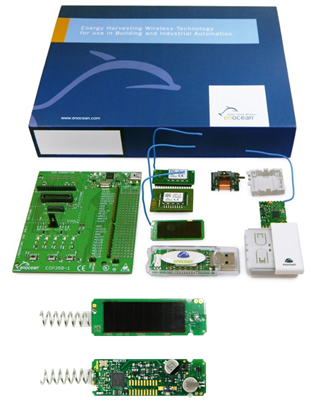
\includegraphics[width=0.9\linewidth,height=5cm]{kitdev.png}
     \caption{Kit de développement}
     \label{dev}
     \end{minipage}\hfill
      \begin{minipage}[c]{0.5\linewidth}
      \centering
     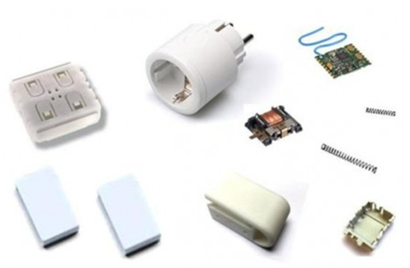
\includegraphics[width=0.7\linewidth,height=5cm]{kitaestetics.png}
     \caption{Kit de design}
     \label{aestetics}
     \end{minipage}\hfill
 \end{figure}


 
\part{Étude}
 \paragraph{Objectifs:}  A partir des éléments disponibles l'analyse s'est concentrée sur la caractérisation et la compréhension des systèmes de récupération d'énergie ainsi que la communication entre les modules et enfin la vérification des critères de portées des communications.
 
 \section{Récupération d'énergie}
 Une partie importante de l'analyse de ce système est l'analyse des technologies de récupération d'énergie. Dans les modules mises à disposition deux technologies sont utilisées, l'une utilise un transducteur mécanique-électrique et l'autre optique-électronique. Le premier dispositif étudié est le convertisseur mécanique-électrique présent dans les interrupteurs de commande.
 
 \subsection{Transducteur Mécanique-électrique}
 
 L'alimentation des interrupteurs sans fils est un circuit magnétique (aimant, fer et bobine, figure \ref{photocircuitmag}) dont la polarité de l'aimant peut être inversée grâce à une languette actionnée par l'utilisateur lorsqu'il presse le bouton (Figure \ref{schemacircuitmag}) il y a donc une partie mobile (en bleu et vert sur la figure \ref{schemacircuitmag} et une partie fixe dont l'aimant fait parti.
 
 \vspace{0.5cm}
 
\begin{figure}[h!]
 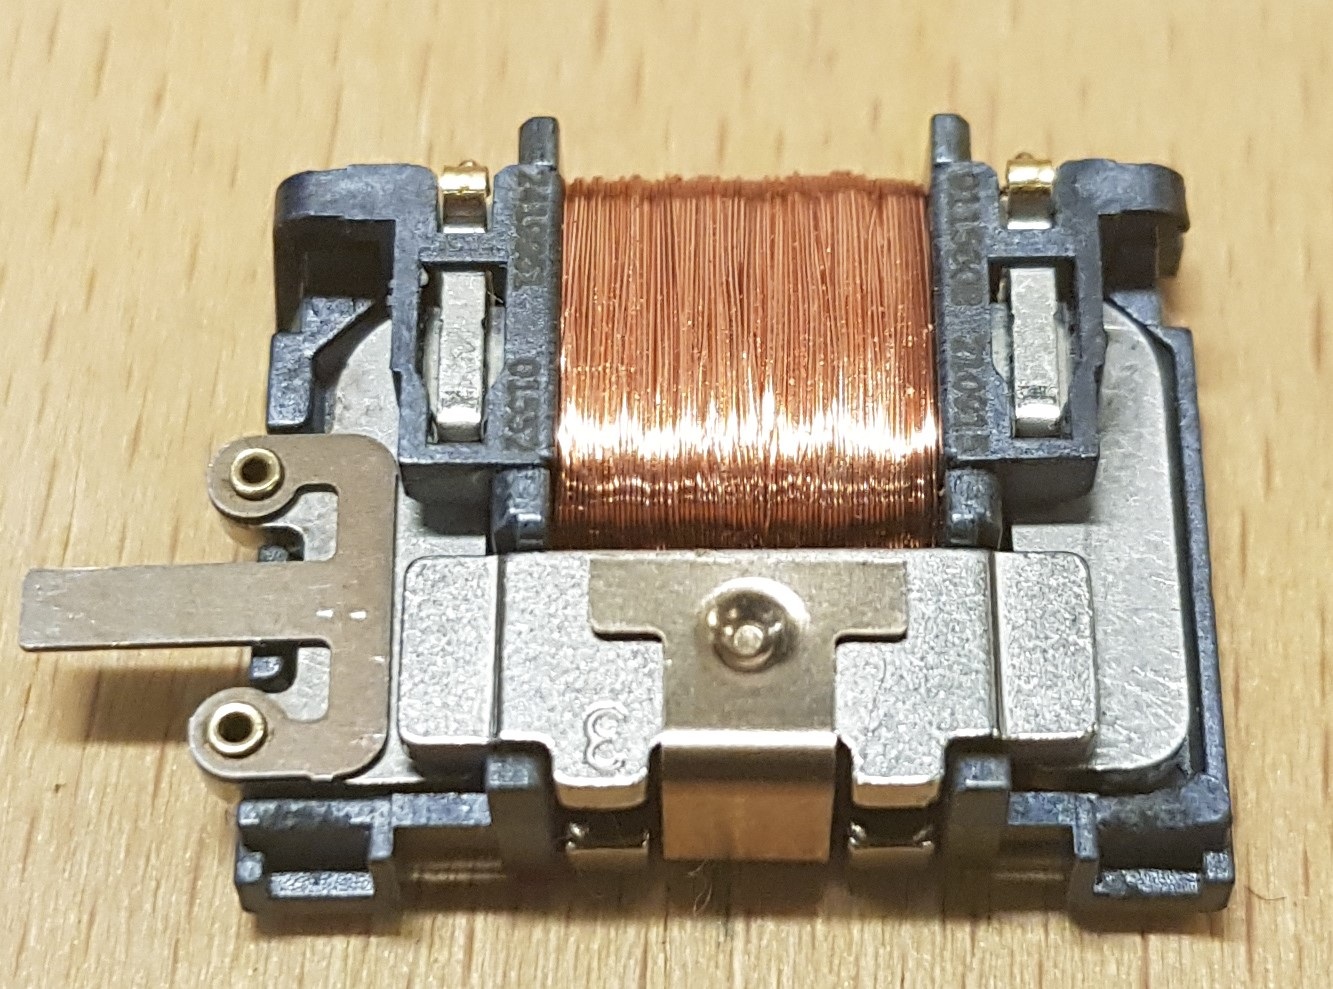
\includegraphics[width = .3\linewidth]{circuitmag.jpg}
 \centering
 \vspace{0.2cm}
 \caption{Circuit magnétique alimentant les interrupteurs sans piles}
 \label{photocircuitmag}
\end{figure}
 \vspace{0.5cm}
 
\begin{figure}[ht!]
 \begin{subfigure}{.5\linewidth}
 \centering
 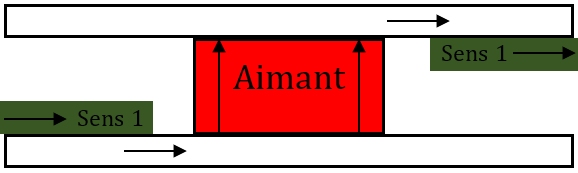
\includegraphics[width=.9\linewidth]{sens1.PNG}
 \vspace{0.2cm}
 \caption{Sens 1 - direct}
 \label{sens1}
 \end{subfigure}
 \begin{subfigure}{.5\linewidth}
 \centering
 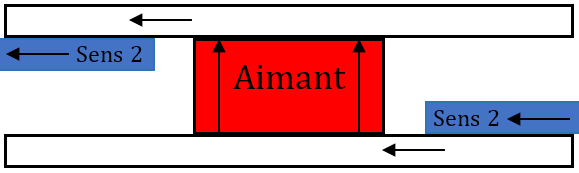
\includegraphics[width=.9\linewidth]{sens2.PNG}
 \vspace{0.2cm}
 \caption{Sens 2 - inversé}
 \label{sens2}
 \end{subfigure}
 \vspace{0.2cm}
 \caption{Différentes positions du circuit magnétique}
 \label{schemacircuitmag}
\end{figure}
 
 \subsubsection{Mesures et expériences}
 
 \subsubsection*{Mesure du pic de tension}
 
 Afin de caractériser le circuit magnétique la première expérience a été d'observer la tension générée aux bornes de la bobine à l'oscilloscope (Figure \ref{tensionobine}). 
 
  \begin{figure}[h!]
 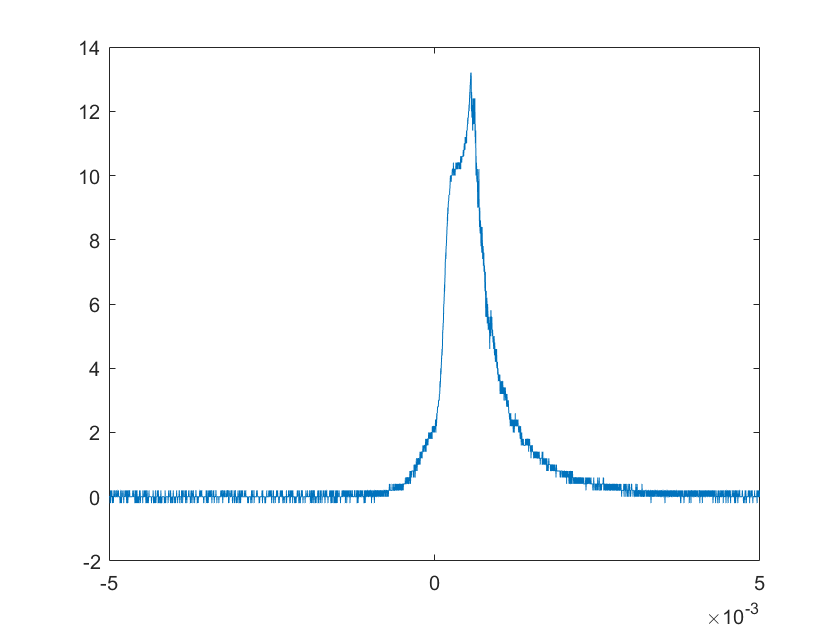
\includegraphics[width = .5\linewidth]{tension.png}
 \centering
 \vspace{0.3cm}
 \caption{Tension ($V$) en fonction du temps ($s$)}
 \label{tensionobine}
 \end{figure}
 
 \subsubsection*{Mesure du nombre de spires}
 
 Le nombre de spires est mesuré en faisant une seconde bobine sur le circuit magnétique dont on connaît le nombre de spires $N_2 = 5$, le rapport des tensions $U_1$ et $U_2$ (figure \ref{nombredespire}) observés aux bornes des bobines sert à retrouver le nombre de spires $N_1$.
 
 \begin{figure}[h!]
  \centering
 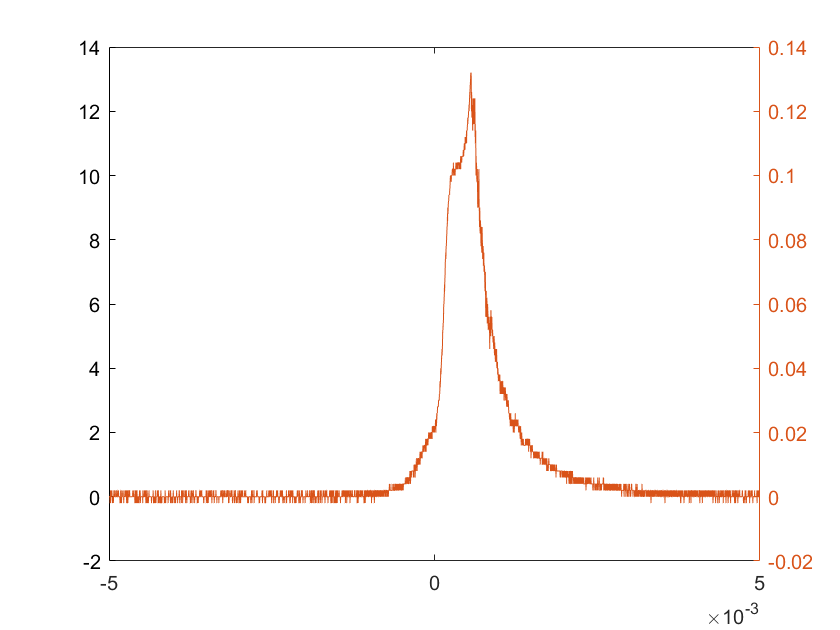
\includegraphics[width = .5\linewidth]{nombredespire.png}
 \vspace{0.3cm}
 \caption{$U_1$ (axe de gauche) et $U_2$ (axe de droite) en fonction du temps $(s)$ superposés}
 \label{nombredespire}
 \end{figure}
 
 \begin{equation}
     \frac{U_1}{U_2} = \frac{N_1}{N_2} \Leftrightarrow N_1 = \frac{U_1\cdot N_2}{U_2} = \frac{13V \times 5}{0,13V} = 500
 \end{equation}
 
 \subsubsection*{Mesure de l'entrefer maximum}
 
 Cette mesure est faite pour avoir une référence lors du calcul de l'entrefer $e$ avec la mesure de tension. Avec le débattement $D$ dans la partie fixe et l'épaisseur $E$ de la partie mobile.
 
 \vspace{0.1cm}
 \begin{equation}
     e_{max} = \frac{D-E}{2} = 1,5\times 10^{-4} m
 \end{equation}
 \vspace{0.1cm}
 
 \subsubsection*{Mesure de l'énergie apportée}
 
 La force appliquée au niveau de la languette est mesurée avec un dynamomètre : $3N$. le déplacement effectué est de $1mm$ au même endroit et donc l'énergie apportée est de :
 
 \vspace{0.1cm}
 \begin{equation}
     E = \overrightarrow{F}\cdot \overrightarrow{dl} = 3N \times 10^{-3}m = 3mJ
 \end{equation}
 \vspace{0.1cm}
 
 Puis la puissance délivrée sur un intervalle de temps de $4\times 10^{-5} s$ est :
 
 \vspace{0.1cm}
 \begin{equation}
     P = \frac{dE}{dt} = \frac{3\times 10^{-3}J}{4\times 10^{-5}s} = 75W
 \end{equation}
 
 \subsubsection{Étude théorique}
 
 Lorsque l'interrupteur est actionné un bref pic de tension est observé aux bornes de la bobine (mesure faite à l'osciloscope, figure \ref{tensionobine}).
 
 Avec ces données le flux total \textit{"vu"} par la bobine avec la Loi de Lenz (Figure \ref{fluxobine}) est :
 
 \vspace{0.1cm}
 \begin{equation}
 \Phi_{tot}(t) = -\int U(t) dt
 \end{equation}
 
 \begin{figure}[h!]
 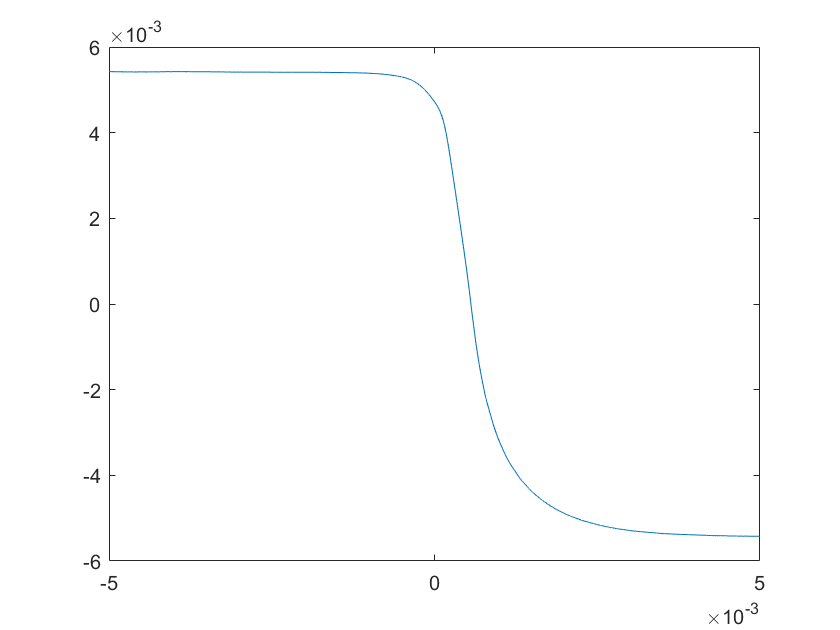
\includegraphics[width = .5\linewidth]{flux.png}
 \centering
 \vspace{0.5cm}
 \caption{Flux ($Wb$) en fonction du temps ($s$)}
 \label{fluxobine}
 \end{figure}
 \vspace{0.5cm}
 
 Puis avec la définition du flux magnétique, le champ magnétique (Figure \ref{champ}) est : 
 
 \vspace{0.1cm}
 \begin{equation}
 \Vert \overrightarrow{B}(t) \Vert = \frac{\Phi_{tot}(t)}{N \cdot dS}
 \end{equation}
 
 \begin{figure}[h!]
 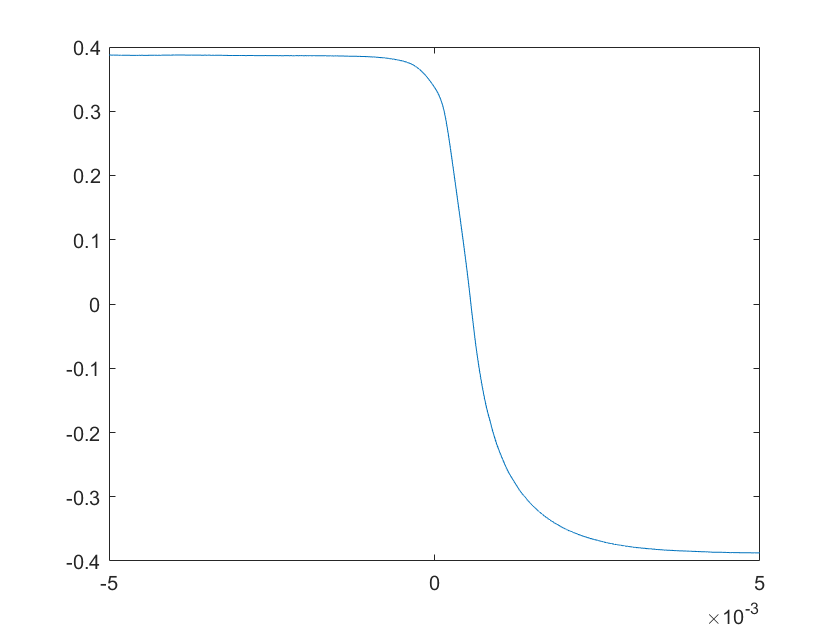
\includegraphics[width = .5\linewidth]{champmag.png}
 \centering
 \vspace{0.5cm}
 \caption{Champ magnétique ($T$) en fonction du temps ($s$)}
 \label{champ}
 \end{figure}
 \vspace{0.2cm}
 
 Avec $N$ le nombre de spires dans la bobine, l'entrefer se déduit en supposant que la perméabilité du fer est très grande devant celle du vide et donc négligeable (Figure \ref{entrefer}) :

 \vspace{0.1cm}
 \begin{equation}
 e(t) = \frac{\mu_0 \cdot dS}{\Phi_{tot}(t)}
 \end{equation}
 
 \begin{figure}[h!]
 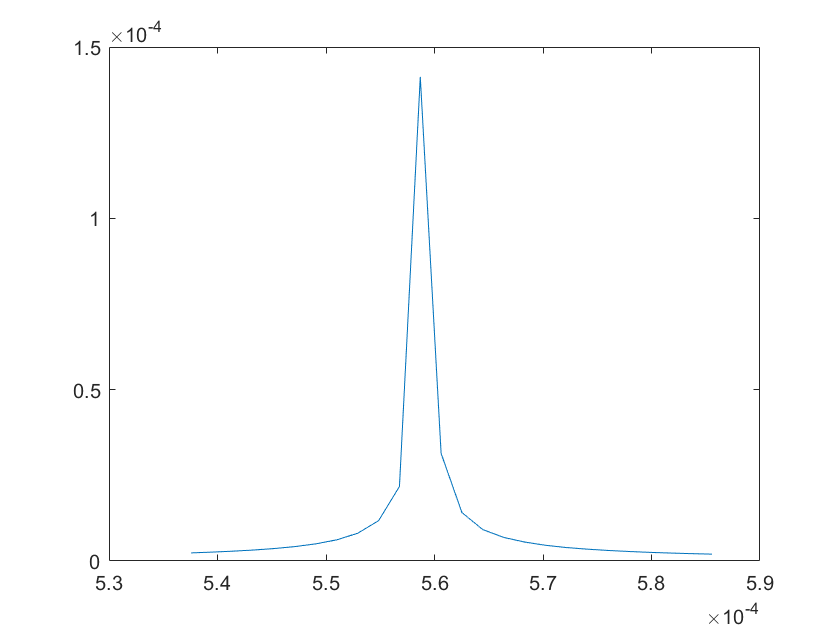
\includegraphics[width = .5\linewidth]{entrefer.png}
 \centering
 \vspace{0.5cm}
 \caption{Entrefer ($m$) en fonction du temps ($s$)}
 \label{entrefer}
 \end{figure}
 \vspace{1cm}
 
 Finalement, pour quantifier le rendement du système, l'énergie magnétique (Figure \ref{energiemag}) s'écrit avec $I_{eq}$ le courant qui génère le même flux $\Phi_{tot}$ que l'aimant sur une spire:
 
 \vspace{0.1cm}
 \begin{equation}
     E = \frac{I_{eq}\times \Phi_{tot}}{2}
 \end{equation}
 \vspace{0.1cm}
 
 Avec $\Phi_{tot} = LI_{eq}$ et $L = \frac{e}{\mu_0 S}$ (Inductance) :
 
 \vspace{0.1cm}
  \begin{equation}
     E = \frac{e I_{eq}^2}{2 \mu_0 S}
 \end{equation}
 \vspace{0.1cm}
 
 \begin{figure}[h!]
 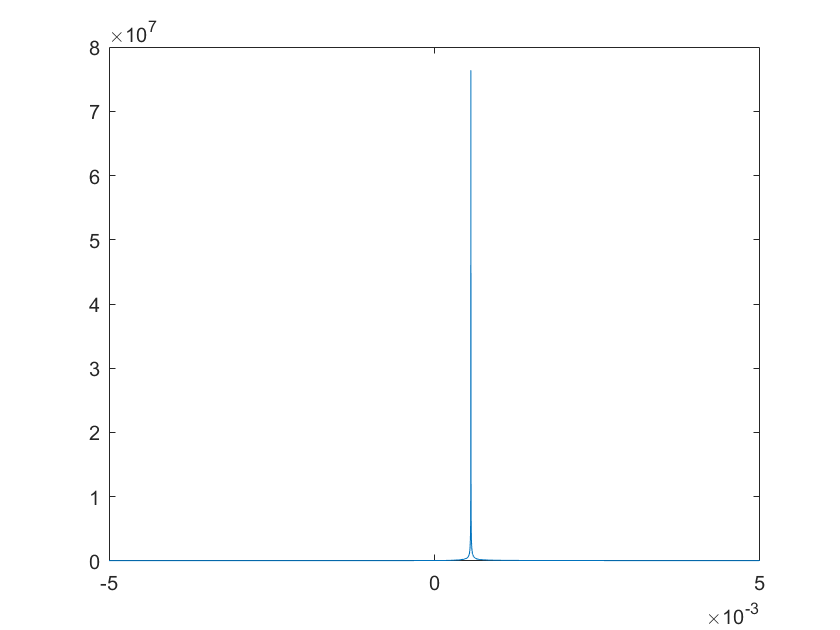
\includegraphics[width = .5\linewidth]{energiemag.png}
 \centering
 \vspace{0.5cm}
 \caption{Energie magnétique ($J$) en fonction du temps ($s$)}
 \label{energiemag}
 \end{figure}
 \vspace{0.2cm}
 
 Avec un rendement calculé de $250\times 10^{9}$, ce résultat n'a aucun sens et ne correspond pas à la valeur attendue. Il n'a malheureusement pas été possible de contacter un professeur afin de vérifier le raisonnement adopté.
 
 \subsubsection{Conclusion}
 
 Malgré la valeur de l'énergie magnétique calculée beaucoup trop grande, la puissance mécanique apportée $(75W)$ est supérieure de plusieurs ordres de grandeur à celle nécessaire pour une bonne transmission de l'information $(\approx 1nW)$. Ainsi l'alimentation pourrait théoriquement avoir un rendement en dessous du $\%$ tout en remplissant bien le cahier des charges proposé (Figure \ref{tableau_cdcf}).
 
 \subsection{Convertisseur optique-électronique}
 \paragraph{Énergie disponible}
 Si l'on considère en première approximation que l'éclairage d'une pièce fournie environ $6W/m^2$, un panneau solaire de surface $5cm$ x $1cm$  avec un rendement de $20\%$ fournit alors une puissance instantanée disponible de l'ordre du milliWatt. Ce qui sur une journée représente une énergie disponible suffisante au vue des puissances nécessaires annoncer par le constructeur inférieur au milliWatt.
 
 \subsubsection{Théorie sur les panneaux solaires}
D'après la théorie sur un modèle (Figure \ref{fig:schema_pv}),le panneau solaire peut être représenté par un générateur de courant dont le courant fourni ($Icc$) est proportionnel à la surface éclairée et à l'irradiance. De plus il y  a une diode en parallèle qui représente le courant dans le noir dû en partie à des effets thermiques ($Vd$) puis une résistance en parallèle ($R_{SH}$) et une en série ($R_{S}$) fixant la tension à vide et la tension en court circuit du panneau solaire.\\

\begin{figure}[h!]
    \centering
    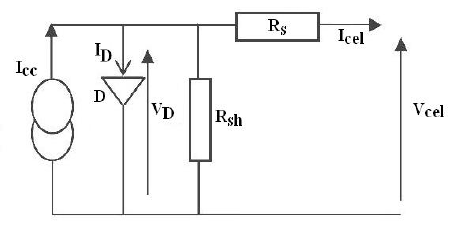
\includegraphics[width=0.9\linewidth]{schema_pv.png}
    \vspace{0.5cm}
    \caption{Schéma électrique équivalent d'un panneau solaire}
    \label{fig:schema_pv}
\end{figure}

Ce modèle permet de tracer la caractéristique d'un panneau solaire ($I_{cel}$ en fonction de $V_{cel} $). Cette caractéristique montre une tension constante puis tombe rapidement à zéro à l'approche du courant de court circuit et la tension est nulle lorsque que le courant de court circuit est atteint (Figure \ref{fig:caracteristique_pv}). De plus ce courant de court circuit évolue avec l'irradiance à l'opposé de la tension en circuit ouvert qui est dépendant très peu de l'irradiance.

\begin{figure}[h!]
    \centering
    \vspace{0.5cm}
    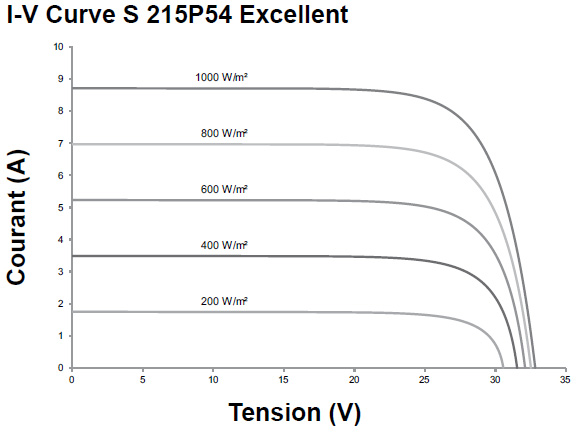
\includegraphics[width=0.7\linewidth]{caracteristique_pv.jpg}
    \caption{Caractéristique théorique d'un panneau solaire}
    \label{fig:caracteristique_pv}
\end{figure}

La théorie et le calcul grossier de puissance disponible permettent de justifier l'utilisation d'un panneau solaire pour servir d'alimentation au dispositif \textit{EnOcean} au vue des puissances annoncées par le constructeur.

 \subsubsection{Choix du constructeur}
 Les panneaux solaires sont utilisés par le constructeur sur les capteurs(Figure \ref{fig:capteur_pv}) afin de remplir la fonction de contraintes sur la récupération d'énergie. Les caractéristiques du panneau solaire monté sur ces capteurs sont disponibles dans la documentation technique du fabricant. La puissance maximale d'un panneau solaire étant inférieur à $V_{operating} \cdot I_{operating} =3\cdot 4.5\cdot 10^{-6} = 14\mu W$ . La valeur maximale de puissance est donc inférieure aux valeurs annoncées par le constructeur.
 
 \begin{figure}[h!]
     \centering
      \begin{minipage}[c]{0.5\linewidth}
      \centering
     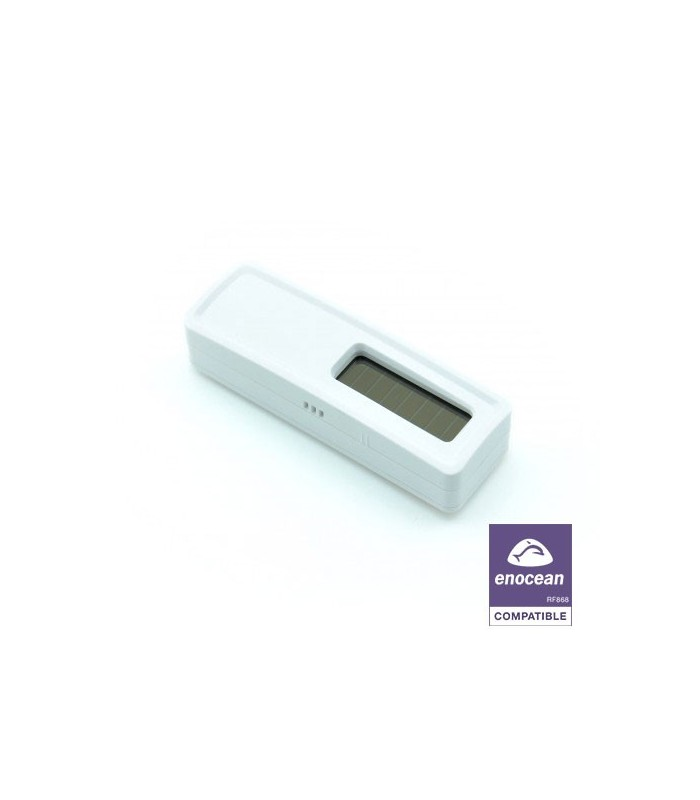
\includegraphics[width=0.7\linewidth,height=5cm] {capteur_pv.jpg}
     \caption{Capteur de température \textit{Enocean} utilisant un panneau solaire}
     \label{fig:capteur_pv}
     \end{minipage}\hfill
      \begin{minipage}[c]{0.5\linewidth}
      \centering
     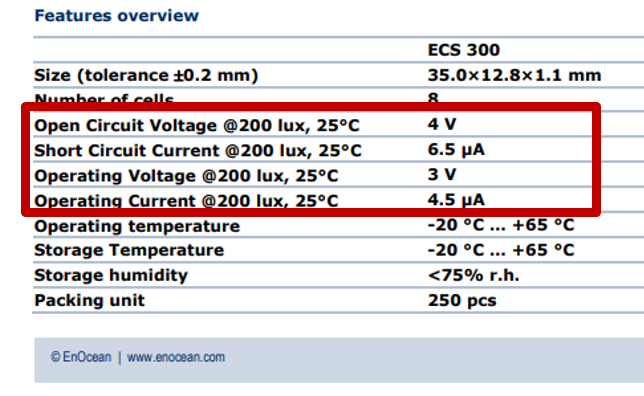
\includegraphics[width=0.9\linewidth,height=5cm]{doc_pv.png}
     \caption{Documentation technique  \textit{Enocean}}
     \label{fig:doc_pv}
     \end{minipage}\hfill
 \end{figure}
 
 \subsubsection{Expérience}
 Une expérience a été réalisé afin de vérifier les caractéristiques du panneau solaire proposé par le fabricant. Le problème pour une expérience sur ce panneau est que les valeurs de courants à mesurer sont beaucoup trop faibles par rapport à la précision des instruments disponibles. L'étude a donc été faite sur un panneau solaire plus grand et une loi d'échelle permettra de raccrocher l'expérience au panneau du constructeur.
 
  \subsubsection*{Protocole}
 Le protocole choisit est de brancher le panneau solaire en parallèle d'un condensateur afin de lisser les valeurs puis sur un bras de pont piloté avec un rapport cyclique $\alpha$. Entre le point milieu du bras de pont et la masse du circuit, il y a une charge formée par une résistance et une bobine connecté. Avec ce montage (Figure \ref{fig:exp}) si on fait varier le rapport cyclique du bras de pont, la résistance vue par le panneau solaire varie. Ceci permet donc de parcourir une grande partie de la caractéristique du panneau solaire. Les caractéristiques du panneau solaire dépendant aussi de l'irradiance celle-ci sera mesurée par un luxmètre. L'expérience a été réalisée sous trois éclairements, 1 du soleil et 2 en intérieur sous des lumières artificielles.
 
 \begin{figure}[h!]
     \centering
     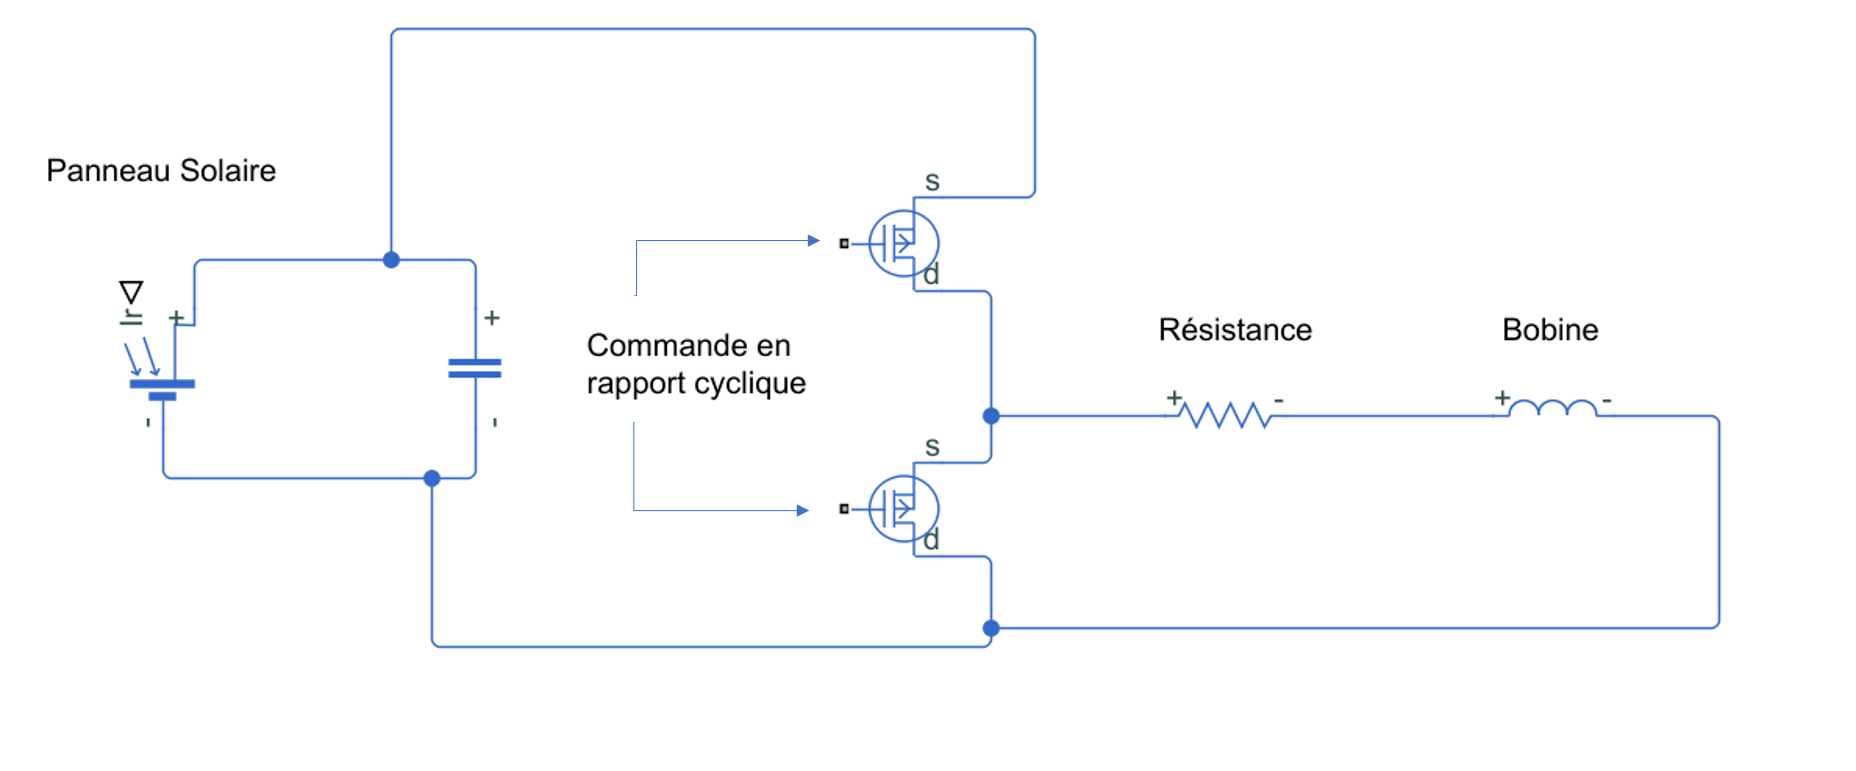
\includegraphics[width=0.9\linewidth]{exp_montage.png}
     \caption{Montage de l'expérience}
     \label{fig:exp}
 \end{figure}
 
 \subsubsection*{Résultats}
 
 A partir des mesures réalisées lors de l'expérience, la caractéristique du panneau solaire(figure \ref{fig:plot_exp} ) mise en évidence est analogue à la théorie à ceci prés que le courant de court circuit n'est pas linéaire avec l'irradiance.
 
 \begin{figure}[h!]
     \centering
     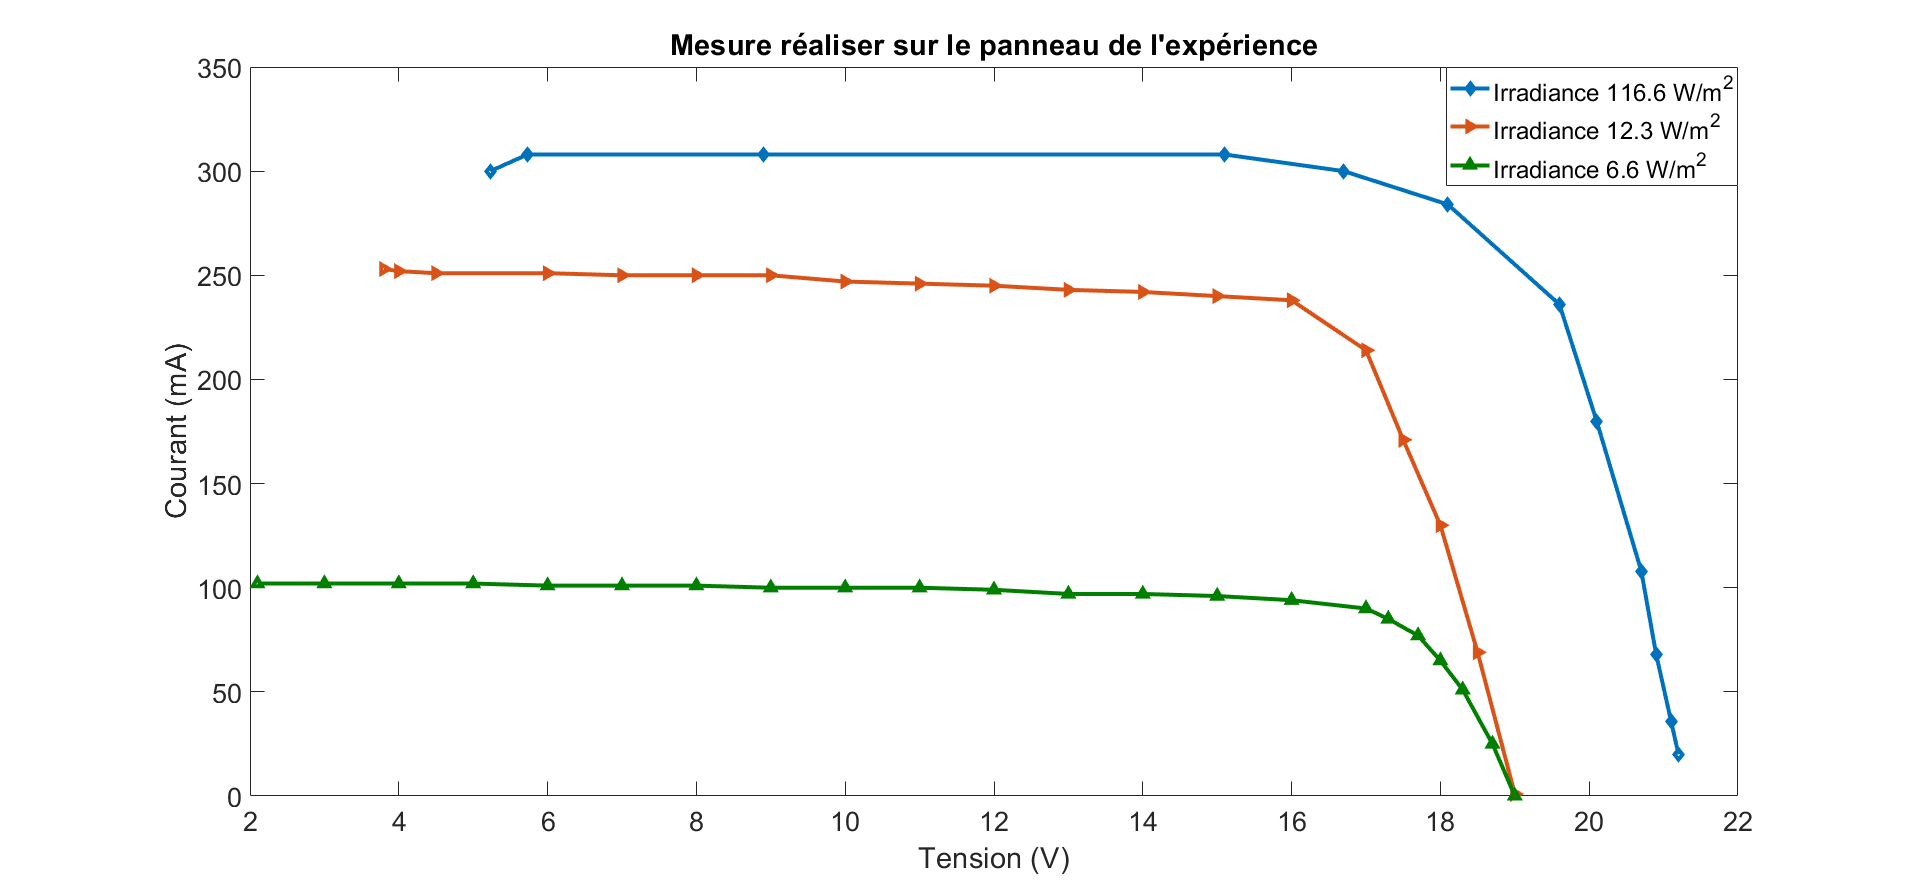
\includegraphics[width=\linewidth]{plot_exp.png}
     \caption{Caractéristique du panneau solaire utilisé pour l'expérience}
     \label{fig:plot_exp}
 \end{figure}
 
 
 \paragraph{Exploitation} Une loi d'échelle permet de raccrocher les valeurs mesurées aux valeurs fournies par les panneaux solaire présent sur les modules \textit{EnOcean}. Ceci en ramenant la tension en circuit ouvert à celle donnée dans la documentation, puis en appliquant le rapport des surfaces éclairées sur le courant, afin de se rapprocher de la caractéristique supposée du panneau solaire fournit par le fabriquant (figure \ref{fig:plot_enocean}).
 
 \begin{figure}[h!]
     \centering
     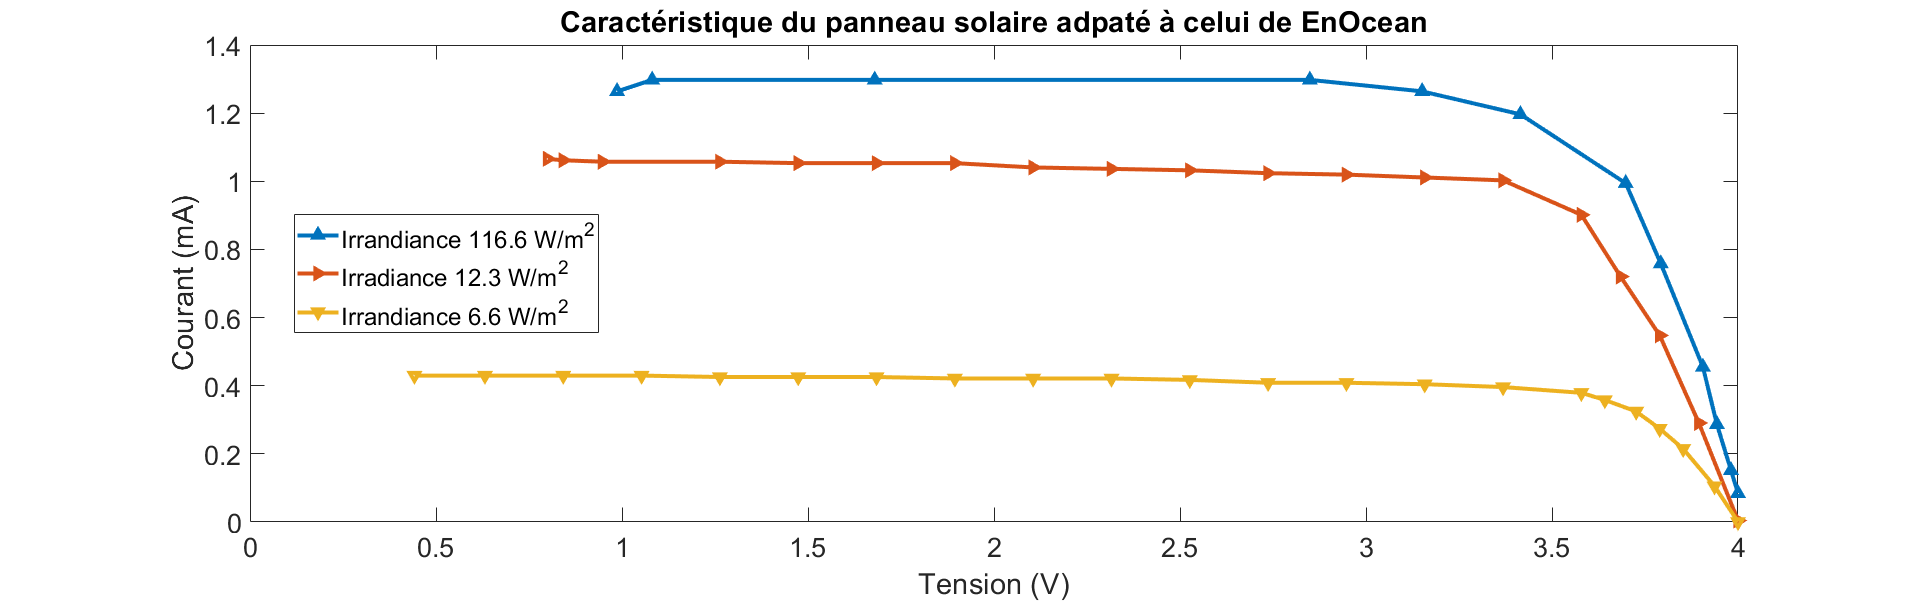
\includegraphics[width=\linewidth]{plot_enocean.png}
    \vspace{0.3cm}
     \caption{Caractéristique du panneau solaire mise à l'échelle}
    \vspace{0.5cm}
     \label{fig:plot_enocean}
 \end{figure}
 
 \paragraph{Analyses} La non linéarité  peut s'expliquer par la répartition spectrale de la source lumineuse (figure  \ref{fig:spectre_soleil}-\ref{fig:halogène}) car le silicium répond de manière différente en fonction de la longueur d'onde de la lumière incidente (figure \ref{fig:silicium}).
 
  \begin{figure}[h!]
     \centering
      \begin{minipage}[c]{0.5\linewidth}
      \centering
     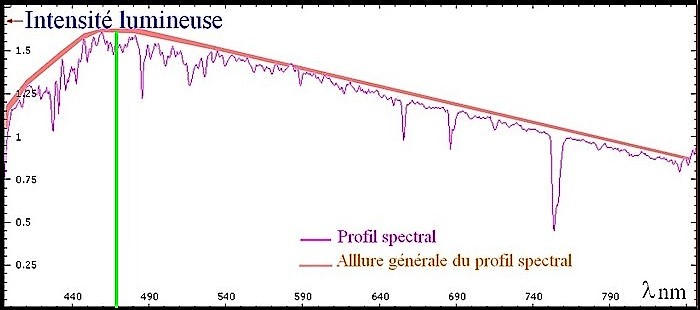
\includegraphics[width=0.9\linewidth,height=5cm]{spectre_soleil.jpg}
    \vspace{0.5cm}
     \caption{Spectre du soleil}
    \vspace{0.5cm}
     \label{fig:spectre_soleil}
     \end{minipage}\hfill
      \begin{minipage}[c]{0.5\linewidth}
      \centering
     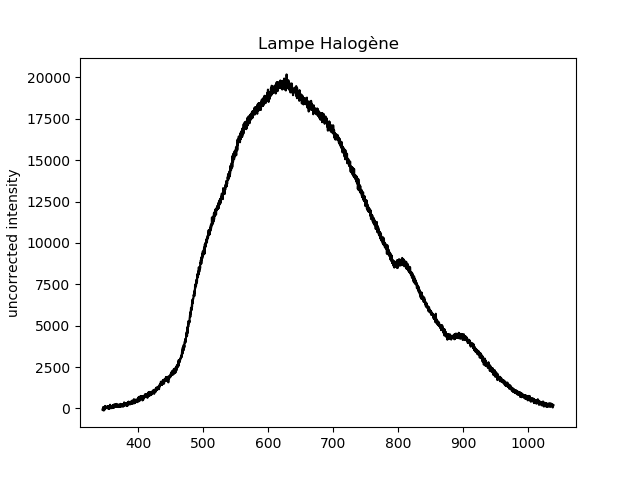
\includegraphics[width=0.9\linewidth,height=5.5cm]{halogene.png}
    \vspace{0.5cm}
     \caption{Spectre lampe d'intérieur halogène utilisé pour l'expérience}
    \vspace{0.5cm}
     \label{fig:halogène}
     \end{minipage}\hfill
     
 \end{figure}
 
 \begin{figure}[h!]
     \centering
     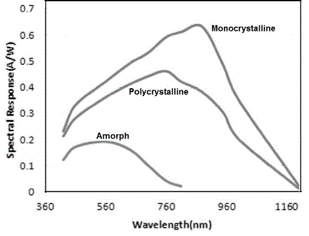
\includegraphics [scale=1]{silicium.png}
    \vspace{0.5cm}
     \caption{Réponse spectrale du silicium en fonction de la technologie et de la longueur d'onde}
     \label{fig:silicium}
 \end{figure}

Le courant de court-circuit a aussi une différence par rapport à la loi d'échelle. En convertissant sans précision sur la longueur d'onde les $200 lux$ en $W/m^2$ puis avec une relation de proportionnalité entre le courant et l'irradiance, la valeur du courant de court circuit serait donc $20\mu A$ sous $200  lux$ pour une valeur attendue de $6.5\mu A$,  soit un écart relatif de $208\%$. Cet écart peut être du à la différence technologique entre le panneau étudié (polycristalin) et  le panneau du kit (monocristalin) ainsi qu'aux sources utilisées pour les mesures car il y a un manque d'information sur les $200 lux$ annoncés notamment sur la longueur d'onde utilisée lors de la mesure par le fabriquant. 
 
 \subsubsection{Conclusion}
 La conclusion de cette étude sur le panneau est qu'il y a des problèmes lors de la loi d'échelle et un manque d'information sur la mesure effectuée par le fabriquant. Malgré cela, si le panneau solaire suit une caractéristique proche de celle mise à l'échelle alors le panneau solaire suffit à fournir la puissance voulue pour le fonctionnement des dispositifs utilisant cette technologie pour la récupération d'énergie.
 
 \section{Réseaux}
 \subsection{Réseaux}
 \subsubsection{Type de réseaux}
 
 Les dispositifs \textit{EnOcean} permettent de créer des réseaux étoilés indépendants entre des actionneurs et les commandes, mais aussi une partie de réseaux maillés avec des répéteurs spécifiques (2 sauts maximum) et les communications avec les passerelles de contrôle qui peuvent faire le lien entre des valeurs de capteurs et des actionneurs.
 
 Lorsqu'un nouveau dispositif apparaît sur le réseau celui-ci envoie une trame afin de se faire identifier et ainsi permettre à la passerelle de comprendre les données qui seront transmises par la suite.
 
 \begin{figure}[h!]
     \centering
     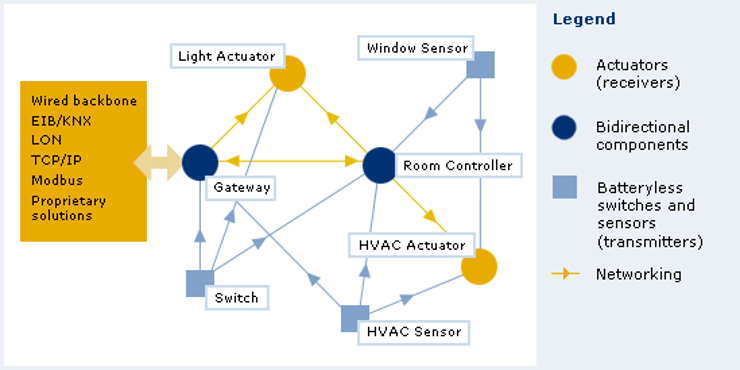
\includegraphics[width=\linewidth]{resseaux.png}
     \caption{Schéma du réseau}
     \label{fig:resseaux}
 \end{figure}
 
 \subsubsection{Protocoles}
 Le protocole de transmission sans fils utilisé par \textit{EnOcean} est un protocole développé par \textit{EnOcean} pour les besoins de ces kits de domotique avec récupération d'énergie. Ce protocole est à l'origine d'une norme pour les ensembles domotiques similaires: ISO/IEC 14543-3-10. Ce protocole définit que les communications sont très courtes et souvent unidirectionnelles ainsi que les fréquences utilisées en fonction de la région du monde ($868 Mhz$ pour l'Europe et la Chine et $315Mhz$ pour les États-Unies et le Japon) afin de limiter les interférences et assurer une bonne portée pour l'utilisation. Au vu des faibles puissances en jeu seule la modulation de fréquence peut permettre de transmettre un message malgré le bruit ambiant. 
 
 \subsection{Caractéristique de la transmission sans fils}
 \subsubsection{Protocole et Théorie}
La transmission sans fils peut être caractérisée par la puissance du signal reçu. Dans cet objectif une expérience avec un émetteur émettant un signal toutes les $0.5 s$ et un récepteur mobile. En connaissant la distance entre les deux cela permet de tracer la puissance reçue en fonction de la distance(figure \ref{fig:exp_sans_fils} ). 

\begin{figure}[h!]
    \centering
    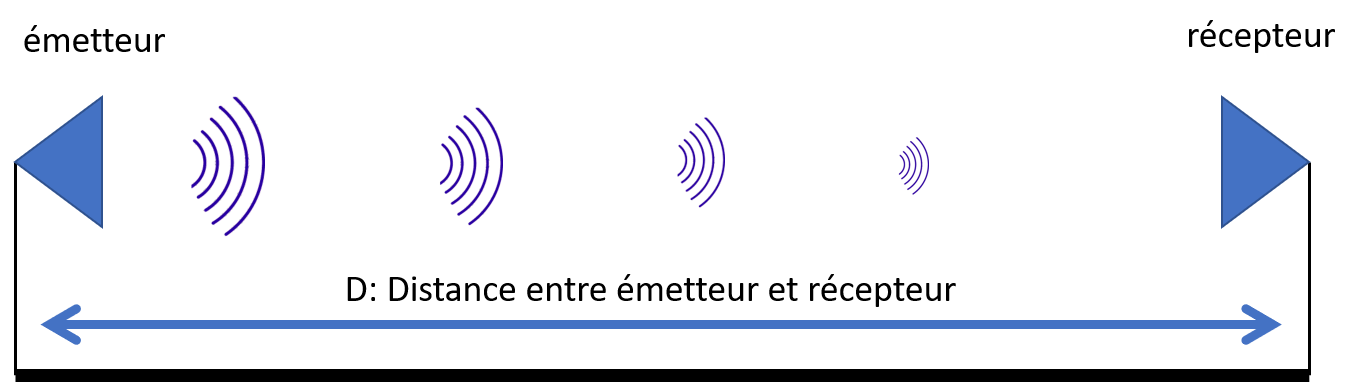
\includegraphics[width=\linewidth,height=5.5cm]{exp_resseaux.png}
    \vspace{0.5cm}
    \caption{schéma de l'expérience sur la transmission sans fils}
    \vspace{0.5cm}
    \label{fig:exp_sans_fils}
\end{figure}

Cette expérience est valable uniquement en champ lointain de l'antenne, ceci se vérifie avec la formule $ R=\frac{2\cdot D^2}{\lambda}$ avec $D$ l'ouverture de l'antenne ici $D=2cm$ au vue des dimensions du dispositif et $\lambda$ la longueur d'onde soit $\lambda=34.56cm$. La zone de champ lointain commence donc à $R = 2.3mm$ de l'antenne.
\vspace{0.3cm}\\
Le logiciel fournit avec les passerelles USB permet d'avoir la puissance du signal reçu en dBm. L'expérience est réalisé entre deux passerelles USB afin d'avoir des gains d'antenne identique et de vérifier la formule de Friis : $P_R=(\frac{\lambda}{4\pi D})^2 G_T G_R P_T $.
\vspace{0.2cm}\\
Dans l'équation de Friis : 
\vspace{0.2cm}
\begin{itemize}
    \item[$P_R$] : Puissance reçue sur l'antenne réceptrice
    \item[$P_T$] : Puissance émise par l'antenne émettrice
    \item[$G_T$] : Gain de l'antenne émettrice
    \item[$G_R$] : Gain de l'antenne réceptrice
\end{itemize}
\subsubsection{Résultats}
Le tracé de la puissance du signal reçu en fonction de la distance(figure \ref{fig:plot_radio}) ressemble à l'équation de Friss ce qui est montrée par l'interpolation.

\begin{figure}[h!]
    \centering
    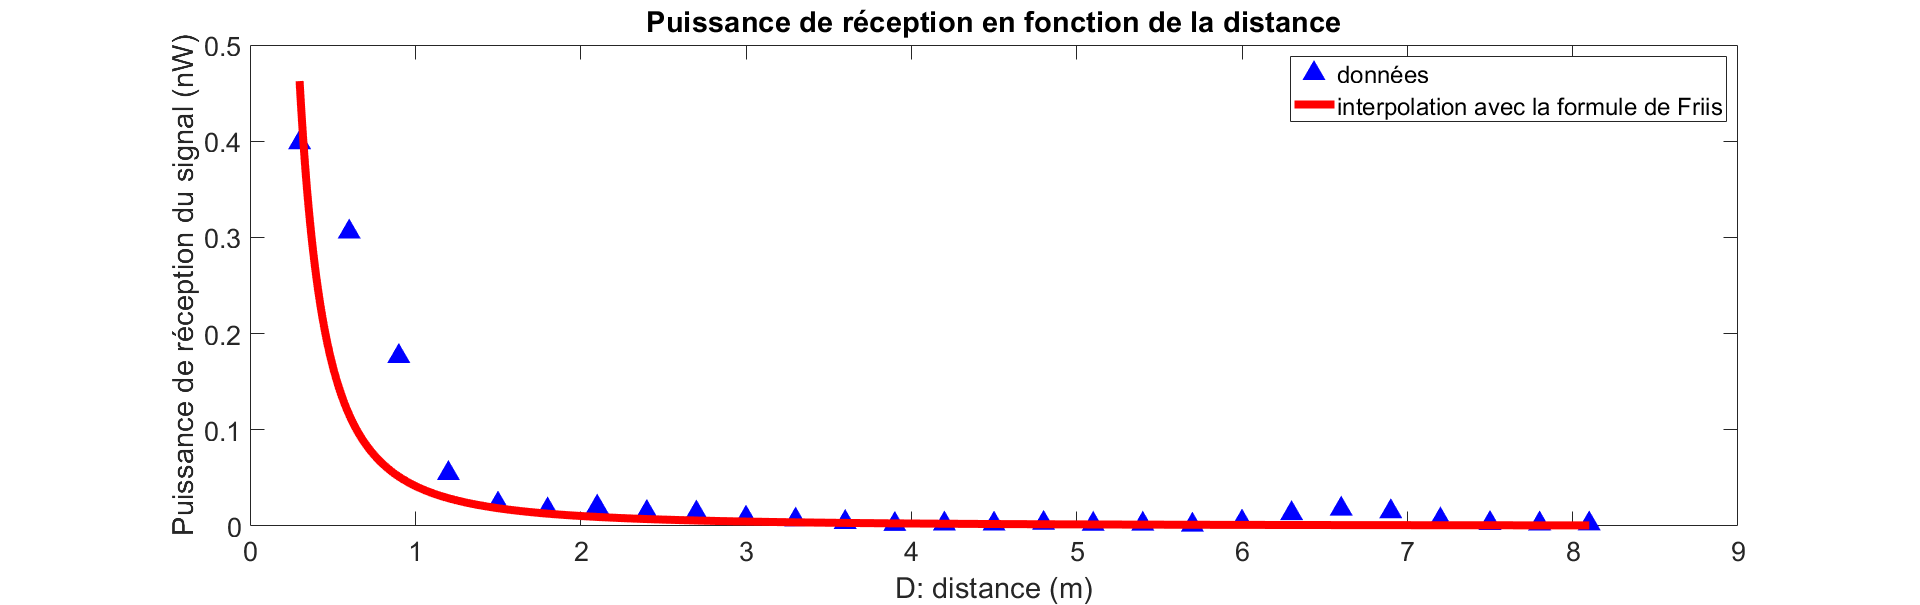
\includegraphics[width=\linewidth]{plot_radio.png}
    \caption{Tracé de la puissance du signal reçu en fonction de la distance}
    \label{fig:plot_radio}
\end{figure}

\subsubsection{Analyse}
L'interpolation diminue bien plus vite que la courbe de mesure.La courbe de mesure semble avoir une périodicité spatiale surtout vers les dernières valeurs de l'acquisition. Cette périodicité et l'écart avec la formule de Friss peut être expliqués avec les multi-chemins possibles car l'étude a été faite dans un milieu avec de nombreuses pièces métalliques qui peuvent donc modifier la propagation de l'onde. \newline
Malgré ces différences, le cas d'utilisation de ces modules dans une habitation montrerait des problèmes similaires car l'environnement serait aussi perturbé. Il est donc quand même possible d'exploiter ces résultats. La distance maximale trouvée est de $11m$ à comparer aux $30m$ annoncé par le constructeur soit un écart relatif de $63\%$. Cette valeur de $11m$ est acceptable pour une utilisation en milieu domestique. 
\newline
Un autre objectif de cette étude est de quantifier la perte au travers d'un mur afin de savoir le nombre maximum de mur que le signal peut traverser avant d'être perdu. Ici la valeur de la puissance perdue au travers d'un mur est de $P_{pertes}=7.7\cdot 10^{-3} nW$ ce qui permet de traverser environ $50$ murs avant de perdre le signal. Là aussi la valeur est acceptable pour un usage domestique. 

\subsection{Conclusion}
L'ordre de grandeur des puissances pour la transmission est plus faible qu'annoncé, de l'ordre du $nW$ contre une puissance des modules annoncée de l'ordre du $mW$. Malgré ceci les performances mesurées sont suffisantes en utilisation domestique afin de satisfaire la fonction principale de  communication de ce kit de domotique. De plus le fonctionnement du réseau permet un ajout simple de nouveaux modules et ne met pas en péril le système entier en cas de défaillance d'un module. Ceci permet de répondre à la facilité d'utilisation et d'installation de cet ensemble étudié.


\part{Conclusion}

Après avoir étudié les modes d'alimentation sans piles ni fils des modules \textit{EnOcean}, les résultats obtenus permettent de vérifier leurs performances vis-à-vis du cahier des charges (Figure \ref{tableau_cdcf}) et ainsi de valider leur choix dans la phase de conception. De plus le réseau de communication permet une facilité d'utilisation et une robustesse face aux mal-fonctions de modules individuels qui est conforme aux attentes du cahier des charges.

Durant les études des difficultés ont été rencontrées notamment pour la caractérisation du panneau solaire au vu du faible niveau des valeurs et de la précision des appareils disponibles ainsi que le manque d'informations sur l'ensemble des technologies déployées par \textit{EnOcean}. Ce manque d'informations se retrouve aussi dans l'étude du réseau car il était impossible d'accéder aux trames émises ou reçues aussi bien de manière matérielle que logicielle pour comprendre l'encodage et vérifier l'hypothèse de modulation de fréquence. De même pour la caractérisation des antennes. Des études supplémentaires sur le panneau solaire avec des appareils de meilleure précision pourraient permettre de vérifier les caractéristiques annoncées par le fabricant.Par ailleurs, la caractérisation des émissions radio des modules à l'aide d'une antenne entièrement connue permettrait de mieux voir les limites du système en termes de distance maximale et d'absorption dans le milieu domestique. Il faudra aussi compléter l'étude du circuit magnétique afin d'obtenir des résultats plus plausibles et de pouvoir conclure sur le rendement de cette nouvelle technique de production d'énergie électrique. 

\part{Bibliographie}

\begin{itemize}
    \item Site internet constructeur sur lequel se trouve les documentations techniques et le catalogue des différents produits \textit{EnOcean} : https://www.enocean.com/en/
    \item Cours de Mr. Hamid Benhamed sur les composants et matériaux électromagnétiques disponible à l'adresse : https://edu.ens-rennes.fr/course/view.php?id=164
    \item Thermal effects investigation on electrical properties of silicon solar cells treated by laser irradiation  par Ali Pourakbar Saffar \& Bahman Deldadeh Barani Iran University of Science and Technology
\end{itemize}

\end{document}
